\documentclass[tikz,border=10pt]{standalone}
\usepackage{pgfplots}
\usepackage{pgfplotstable}
\pgfplotsset{compat=1.18}
\newcommand{\flashspread}{\textsc{FlashSpread}}

\begin{document}
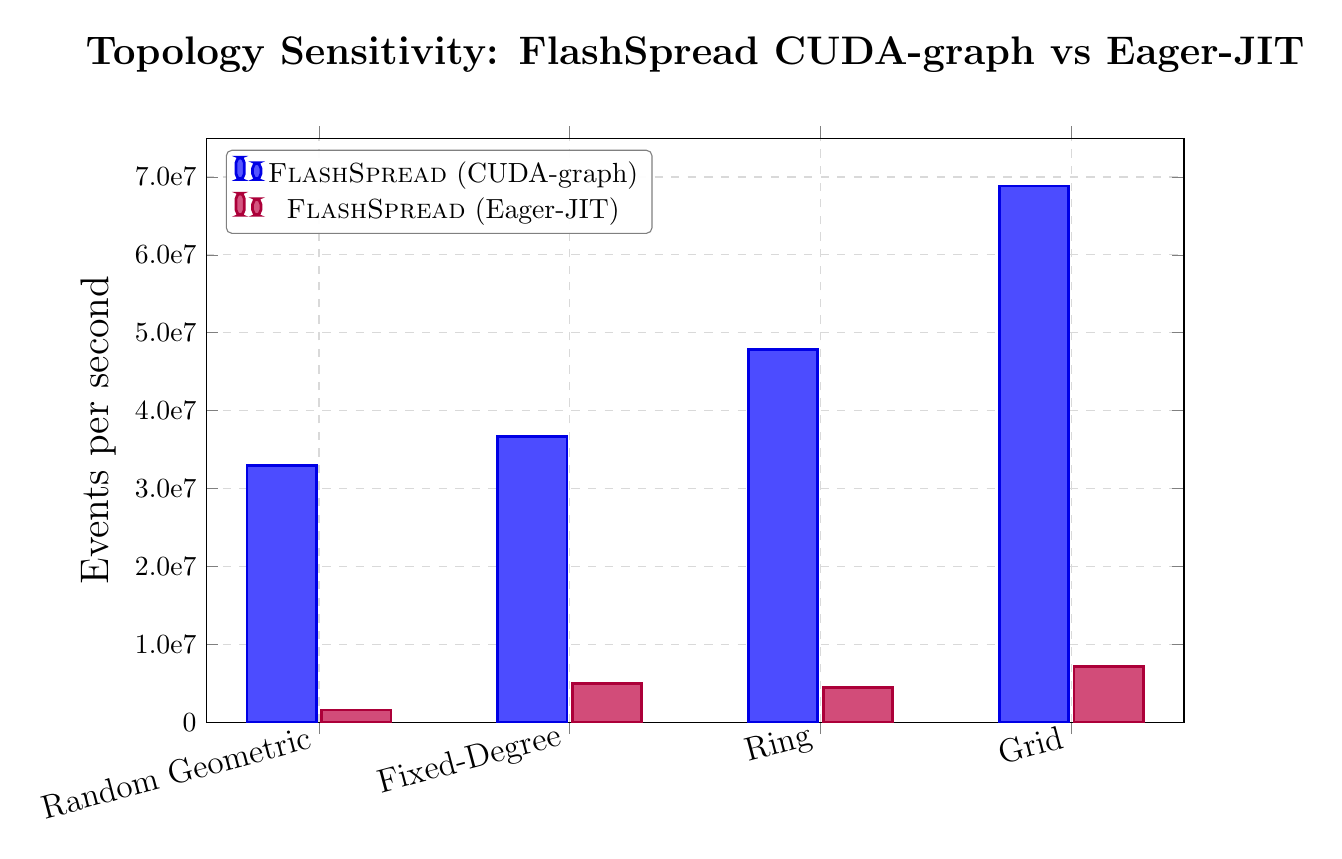
\begin{tikzpicture}
    \begin{axis}[
        ybar,
        bar width=25pt,
        width=14cm,
        height=9cm,
        enlarge x limits=0.15,
        legend style={
            at={(0.02,0.98)},
            anchor=north west,
            legend columns=1,
            font=\normalsize,
            draw=black!50,
            fill=white,
            fill opacity=0.95,
            text opacity=1,
            rounded corners=2pt
        },
        ylabel={Events per second},
        ylabel style={font=\Large},
        symbolic x coords={Random Geometric, Fixed-Degree, Ring, Grid},
        xtick=data,
        xticklabel style={font=\large, rotate=15, anchor=east},
        yticklabel style={
            font=\normalsize,
            /pgf/number format/.cd,
            fixed,
            fixed zerofill,
            precision=1,
            /pgf/number format/1000 sep={}
        },
        scaled y ticks=false,
        ymin=0,
        ymax=7.5e7,
        ytick={0,10000000,20000000,30000000,40000000,50000000,60000000,70000000},
        yticklabels={0,1.0e7,2.0e7,3.0e7,4.0e7,5.0e7,6.0e7,7.0e7},
        grid=major,
        grid style={dashed,gray!30},
        title={Topology Sensitivity: \flashspread{} CUDA-graph vs Eager-JIT},
        title style={font=\Large\bfseries, yshift=0.5cm}
    ]
    
    % CUDA-graph data
    \addplot[
        fill=blue!70,
        draw=blue!90!black,
        line width=1pt
    ] coordinates {
        (Random Geometric, 32919687.75)
        (Fixed-Degree, 36680490.09)
        (Ring, 47844572.30)
        (Grid, 68835139.15)
    };
    
    % Eager-JIT data
    \addplot[
        fill=purple!70,
        draw=purple!90!black,
        line width=1pt
    ] coordinates {
        (Random Geometric, 1551571.97)
        (Fixed-Degree, 4998949.99)
        (Ring, 4444186.38)
        (Grid, 7184217.11)
    };
    
    \legend{\flashspread{} (CUDA-graph), \flashspread{} (Eager-JIT)}
    
    \end{axis}
\end{tikzpicture}
\end{document}